\documentclass[10pt,a4paper]{amsart}
\usepackage{amsmath,amssymb,amsthm,graphicx}
%\usepackage{amsthm}
\usepackage{amsmath}
\usepackage{amssymb}
\usepackage{amsthm}
\usepackage{array}
\usepackage{xy}
\usepackage{hyperref}
\usepackage{color}
\usepackage{latexsym} 
\theoremstyle{plain}
  \newtheorem{theorem}{Theorem}[section]
  \newtheorem{lemma}{Lemma}[section]
  \newtheorem{proposition}{Proposition}[section]
  \newtheorem{question}{Question}[section]
  \newtheorem{corollary}{Corollary}[section]
  \newtheorem{definition}{Definition}[section]
  \newtheorem{remark}{Remark}[section]
  \newtheorem{example}{Example}[section]
  \newtheorem{note}{Note}[section]
  \newtheorem{exercise}{Exercise}[section]
\newcommand{\y}{\bar{y}}
\newcommand{\U}{\bar{u}}
\newcommand{\z}{\bar{c}}

   \newcommand{\beqn}{\begin{eqnarray}}
   \newcommand{\eeqn}{\end{eqnarray}}
   \newcommand{\beqs}{\begin{eqnarray*}}
   \newcommand{\eeqs}{\end{eqnarray*}}
   \newcommand{\ban}{\begin{eqnarray*}}
   \newcommand{\nan}{\end{eqnarray*}}
   \newcommand{\beq}{\begin{equation}}
   \newcommand{\eeq}{\end{equation}}
   
   \newcommand{\p}{\partial}
\newcommand{\eps}{\varepsilon}
\newcommand{\Lm}{\Omega^*}
\newcommand{\Om}{\Omega}
\newcommand{\pom}{{\p\Om}}
\newcommand{\bom}{{\overline\Om}}

  \newcommand{\osc}{{\mbox{osc}}}
\renewcommand{\det}{\mbox{det}}
  \newcommand{\mes}{\mbox{mes}}
  \newcommand{\dist}{\mbox{dist}}
  \newcommand{\diam}{{\mbox{diam}}}
    \newcommand{\rad}{{\mbox{radius}}}
  \newcommand{\diag}{{\mbox{diag}}}
  \newcommand{\Vol}{{\mbox{Vol}}}
  \newcommand{\arctg}{{\mbox{arctg}}}
  \newcommand{\supp}{{\mbox{supp}}}

\newcommand{\ol}{\overline}
\newcommand{\ul}{\underline}
\newcommand{\lan}{\langle}
\newcommand{\ran}{\rangle}
\newcommand{\D}{\nabla}  

\newcommand{\s}{\tilde{v}}
\newcommand{\e}{\varepsilon}
\newcommand{\R}{\mathbb{R}}
\newcommand{\0}{\textbf{0}}
\numberwithin{equation}{section}
\DeclareMathOperator{\cexp}{c-exp}
\DeclareMathOperator{\cstarexp}{c*-exp}

%    Absolute value notation
\newcommand{\abs}[1]{\lvert#1\rvert}

%    Blank box placeholder for figures (to avoid requiring any
%    particular graphics capabilities for printing this document).
\newcommand{\blankbox}[2]{%
  \parbox{\columnwidth}{\centering
%    Set fboxsep to 0 so that the actual size of the box will match the
%    given measurements more closely.
    \setlength{\fboxsep}{0pt}%
    \fbox{\raisebox{0pt}[#2]{\hspace{#1}}}%
  }%
}


%%%%%%%%%%%%%%%%%%%%%%%
\renewcommand{\theequation}{\arabic{section}.\arabic{equation}}
%\newcommand{\mysection}[1]{\section{#1}\setcounter{equation}{0}}
  \numberwithin{equation}{section}
  \numberwithin{figure}{section}

%\TagsOnRight
%\newcommand{TagsOnRight}
%%%%%%%%%%%%%%%%%%%%%%%%%

\renewcommand{\baselinestretch}{1.00}
\parskip = 0.25in
\title{Two-thirds power decay of the normal width of a centred section at the non-convex transport singular set}
\author{Shibing Chen, Jiakun Liu}
\date{arxiv:2210.13841v4; CC BY 4.0}
\begin{document}
\maketitle
\setcounter{section}{4}
\setcounter{lemma}{1}
\noindent\textit{Editorial note.} The counted statement is the lemma labelled ide1 at source lines 838-844 and the proof environment at source lines 846-874 immediately follows it and is its own proof by adjacency; the lemma is not restated anywhere else in the article.\par\medskip
\noindent\textit{Editorial note.} The retained context is what the statement and its proof name or use: the definition of centred sections and sub-level sets at source lines 322-333, the abbreviation of the centred section at y-zero at source lines 701-703, the strict convexity estimate strictconvex at source lines 710-714 that the retained equivalence refers to, the meaning of the comparison symbol approx at source line 728, the volume and tangential estimates of corollary co21 at source lines 735-750, the equivalence equi0 between sub-level sets and centred sections at source lines 756-764, the width function and its maximising point at source lines 829-836, and the diagram f4.1 at source lines 966-970 that the proof points the reader to by its printed number.\par\medskip
\noindent\textit{Editorial note.} The retained section and lemma counters are set to four and one, so the counted lemma prints with the article's own number Lemma 4.2 and the retained corollary prints as Corollary 4.1; the retained definition, which comes from the article's Section 2, necessarily prints as Definition 4.1 rather than its article number, and the single numbered equation of the retained excerpt is numbered by the package. The figure prints as Figure 4.1, exactly the number the proof refers to in words.\par\medskip
\noindent\textit{Editorial note.} The article's own preamble is retained with three omissions only: the class line, which the wrapper supplies as amsart at ten point on A4; the pdftex driver option of graphicx at source line 9, which is not this engine's driver; and the transparent package at source line 12, which the production engine's TeX installation does not carry and which no retained line needs, because the command that package provides occurs nowhere in the article except on its own loading line. The wrapper supplies graphicx without a driver option. No macro is invented, no further package is loaded and no author text is changed.\par\medskip
\noindent\textit{Editorial note.} The retained excerpt is reproduced line for line, including the printed slip in the proof that writes e-sub-p where the surrounding argument uses e-sub-q, and including the tangential estimate statement that the author uses without a cross-reference. No mathematics is repaired and no hypothesis is added.\par\medskip
\noindent\textit{Editorial note.} The article's own bibliography is delivered as a flattened thebibliography fragment, so the citations inside the retained context (Caffarelli, and Chen-Liu-Wang on optimal partial transport) resolve inside the package and no undefined citation can arise. Uncited entries of the same bibliography are delivered unchanged with it.\par\medskip
\noindent\textit{Editorial note.} Every retained line is pure ASCII and the single non-ASCII character of the delivered bibliography is an en dash inside an entry title, which the engine's text font contains, so no missing character is reported.\par\medskip
\noindent\textit{Editorial scope.} One original result: the width estimate labelled ide1 (source lines 838-844) with its complete adjacent author proof (source lines 846-874), together with the article's own definitions and estimates that it names (source lines 322-333, 701-703, 710-714, 728, 735-750, 756-764, 829-836) and the diagram f4.1 (source lines 966-970). Theorem t111 and its Section 3 proof chain (source lines 353-679), the theorem main1, the obliqueness proposition uniob and the lemma ests with its proof (source lines 1737-1808) are not counted here and are not used as premises.\par\medskip
\noindent\textit{Allowed standard prerequisites (editorial).}\begin{itemize}
\item Brenier duality for optimal transport into two separated convex targets. The transport potentials u and v are globally Lipschitz convex functions linked by the dual formulas v(y) = sup over x in Omega of (y dot x minus u(x)) and u-sub-i(x) = sup over y in Omega-sub-i-star of (y dot x minus v(y)), the singular set is the interface where u-one and u-two agree, and the target domains Omega-sub-i-star are convex and separated by a hyperplane.. Fixes the objects of the counted statement: the point y-zero is the image of the singular point under the gradient of u-one, Omega-sub-one-star is the target component whose boundary is touched there, and the width is measured inside that component.
\item Caffarelli regularity and the geometry of centred sections. Under the Monge-Ampere density bounds the centred sections of v are convex, have centre of mass at their centre point, are of geometric decay, and satisfy the strict convexity estimate recalled in the retained context; the volume of a centred section at height h is comparable to h to the power n over two.. The retained volume estimate and the retained tangential estimate are the two inputs of the counted proof, and the retained equivalence between sub-level sets and centred sections converts the width statement into a volume statement.
\item Elementary convex geometry: Hausdorff measure, convex hulls and uniform convexity. The two-dimensional Hausdorff measure of a planar region bounded by a uniformly convex arc and a chord is at least a constant times the three-halves power of the chord height, the convex hull of that region with points at a controlled tangential distance is contained in any convex set containing both, and on a uniformly convex boundary a displacement in the normal direction is at least a constant times the square of the tangential displacement.. These three elementary facts are the substance of the two halves of the counted proof: the lower bound for the measure of the planar region, and the final uniform convexity inequality relating the tangential width to the normal width.
\end{itemize}\medskip
\begin{definition}\label{defS}
Given a point $y_0\in \mathbb{R}^n$ and a small positive constant $h$, we define the centred sections of the convex function $w$ at $y_0$ with height $h$ as:
\begin{equation}\label{sect}
S^c_{h}[w](y_0) := \left\{y\in\mathbb{R}^n : w(y) < w(y_0) + (y-y_0)\cdot \bar{p} + h\right\},
\end{equation}
where $\bar{p}\in \mathbb{R}^n$ is chosen such that the centre of mass of $S^c_{h}[w](y_0)$ coincides with $y_0$.
Additionally, we define the sub-level set of $w$ at $y_0$ with height $h$ as:
\begin{equation}\label{sub}
S_h[w](y_0) := \left\{y\in \mathbb{R}^n : w(y) < \ell_{y_0}(y) + h\right\},
\end{equation}
where $\ell_{y_0}$ denotes an affine supporting function of $w$ at $y_0$.
\end{definition}

The subsequent analysis for $v$ is in a neighbourhood of $y_0$, which nevertheless also applies to $v$ near $\hat y_0$ analogously. 
Hereafter, for brevity we
denote $S^c_{h}[v](y_0)$ by  $S^c_{h}[v]$. 

Moreover, by \cite[Corollary 2.3]{C96} (see also \cite[Proof of Theorem 1]{C92b}), the function $v$ satisfies a strict convexity estimate of the form:
\begin{equation}\label{strictconvex}
v(y) \geq v(y_0) + Dv(y_0) \cdot (y - y_0) + C |y - y_0|^{1 + a}  \quad \forall\, y \in \overline{\Omega_1^*} \ \text{ near } y_0,
\end{equation}
where $a > 1$ and $C$ are constants.

In the following, the notation $a \approx b$ means that $C^{-1}a \leq b \leq Ca$ for some universal positive constant $C.$  Given a convex domain $D \subset \mathbb{R}^n$, we say that $D$ has a \emph{good shape} if $B_{C^{-1}}(x^*) \subset D \subset B_{C}(x^*)$, where $C$ is a universal positive constant and $x^*$ is the centre of mass of $D$.

\begin{corollary}\label{co21}
The following assertions hold true:
\begin{enumerate}
\item[(i)] \emph{Volume Estimate:}
\begin{equation}\label{vol}
|S_h[v](y_0)\cap \Omega_1^*| \approx |S_h^c[v](y_0)\cap \Omega_1^*| \approx |S_h^c[v](y_0)| \approx h^{\frac{n}{2}}.
\end{equation}
Moreover, for any affine transform $\mathcal{A}$, 
if either $\mathcal{A}(S_h^c[v](y_0))$ or $\mathcal{A}(S_h[v](y_0) \cap \Omega_1^*)$ has a good shape, so is the other one.

\item[(ii)] \emph{Tangential $C^{1,1-\epsilon}$ regularity of $v$:} $\forall$ $\epsilon > 0$, $\exists$ a constant $C_\epsilon$ such that:
\begin{equation}\label{tanc2}
B_{C_\epsilon h^{\frac{1}{2}+\epsilon}}(y_0) \cap \mathcal{H} \subset S_h^c[v](y_0) \quad \forall\, h > 0\text{ sufficiently small}.
\end{equation}
\end{enumerate}
\end{corollary}

\begin{remark}\label{reeq1}
\emph{ By the strict convexity of $v$ (see \eqref{strictconvex}) and the fact that $S^c_h[v]$ is centred at $y_0$,
we have an equivalence relation between $S_h[v]$ and $S^c_{h}[v]$, namely $\forall\,h>0$ small, 
\begin{equation}\label{equi0}
S^c_{b^{-1}h}[v] \cap \Omega_1^*\subset S_h[v] \cap \Omega_1^* \subset S^c_{bh}[v] \cap \Omega_1^*,
\end{equation}
where \( b>1 \) is a constant independent of \( h \). 
The reader is referred to \cite[Lemma 2.2]{CLW1} for a proof. }
\end{remark}


Recall the sub-level set $S_h[v]=S_h[v](y_0)=\{v<h\}$ in \eqref{sub}.
Define the width function
\[
d_e := \sup \left\{ |(y-y_0) \cdot e| : y \in S_h[v] \cap \Omega_1^* \right\}\quad \mbox{ for } e\in\mathbb{S}^{n-1}. 
\]
Let $p_e \in \overline{S_h[v] \cap \Omega_1^*}$ be a point where $|(p_e-y_0) \cdot e| = d_e$. When specifically considering the unit vector $e_1$, we shall denote $p_{e_1}$ simply as $p=(p_1, \cdots, p_n)$.


\begin{lemma}\label{ide1}
For any $\epsilon>0$ small, there exists a constant $C_\epsilon$ such that 
	\[ d_{e_1} \leq C_{\epsilon}h^{\frac{2}{3} - \epsilon}. \]
Moreover, for any unit vector $e \in \mathrm{span}\{e_2, \ldots, e_n\}$,  
	\[ d_e^2 \leq C d_{e_1} \] 
for some universal constant $C$. 
\end{lemma}

\begin{proof}
Let \( p \) be as above. Consider \( q \), the point of intersection between the segment \( \overline{op} \) and \( \partial\Omega_1^* \). 
Since both \( p \) and the origin are in \( \overline{S_h[v]} \), by convexity one has \( q \in \overline{S_h[v]} \). Thus,
\[ q \in \overline{S_h[v]} \cap \partial\Omega_1^*. \]
Recall that \( d_{e_1} = p_1 \). 
As the intersection \( S_h[v] \cap \Omega_1^* \) converges to \( y_0 \) as \( h\rightarrow 0 \), we deduce that \( \frac{q_n}{p_n} \geq \frac{1}{2} \) for sufficiently small \( h \). Consequently,
\[ q_1 \geq \frac{q_n}{p_n} p_1 \geq \frac{1}{2} d_{e_1}. \] 

Define \( e_q := \frac{q - y_0}{|q - y_0|} \). 
Let \( D \subset \mathrm{span}\{e_q, e_1\} \) be the planar region bounded by \( \partial\Omega_1^* \cap \mathrm{span}\{e_q, e_1\} \) and the segment \( \overline{y_0q} \). 
Since \( \partial\Omega_1^*\in C^2 \) is uniformly convex, one has 
	\[ \mathcal{H}^2(D) \geq C|q_1|^{\frac{3}{2}} \geq Cd_{e_1}^{3/2} \] 
for a constant \( C \) independent of \( h \), where \( \mathcal{H}^2(\cdot) \) denotes the 2-dimensional Hausdorff measure, see Figure 4.1.

Select \( \{\tilde{e}_2, \ldots, \tilde{e}_{n-1}\} \) to be an orthonormal basis for the orthogonal complement of \( \mathrm{span}\{e_1, e_p\} \) in \( \mathbb{R}^n \). The tangential \( C^{1, 1-\epsilon} \) estimate of \( v \) asserts that
\[ y_0 + C_\epsilon h^{\frac{1}{2}+\epsilon}\tilde{e}_i \in S^c_{bh}[v] \quad \text{for} \quad i=2, \ldots, n-1, \]
where \( b \) is the constant in \eqref{equi0}.
Define \( G \) to be the convex hull of \( D \) and points \(\{ y_0 + C_\epsilon h^{\frac{1}{2}+\epsilon}\tilde{e}_i, \, i=2, \ldots, n-1 \}\). By convexity, it follows that \( G \subset S^c_{bh}[v] \).

Combining these results and the inclusion $S_h[v]\cap \Omega_1^* \subset S^c_{bh}[v]$, we obtain:
\[
C_\epsilon h^{(\frac{1}{2}+\epsilon)(n-2)}\mathcal{H}^2(D) \leq |G| \leq |S^c_{bh}[v]| \approx h^{\frac{n}{2}},
\]
which in turn implies $|d_{e_1}| \leq C_{\epsilon}h^{\frac{2}{3} - \epsilon}$.

Fix any unit vector $e \in \mathrm{span}\{e_2, \ldots, e_n\}$. The uniform convexity of $\partial\Omega_1^*$ yields 
	\[ d_{e_1} \geq (p_e-y_0) \cdot e_1 \geq C_1((p_e-y_0) \cdot e)^2 = C_1d_e^2  \]
for some universal constant $C_1>0$, which implies $d_e^2 \leq C d_{e_1}$ for a universal constant $C$.
\end{proof}

\begin{figure}[h]\label{f4.1}
 \centering
 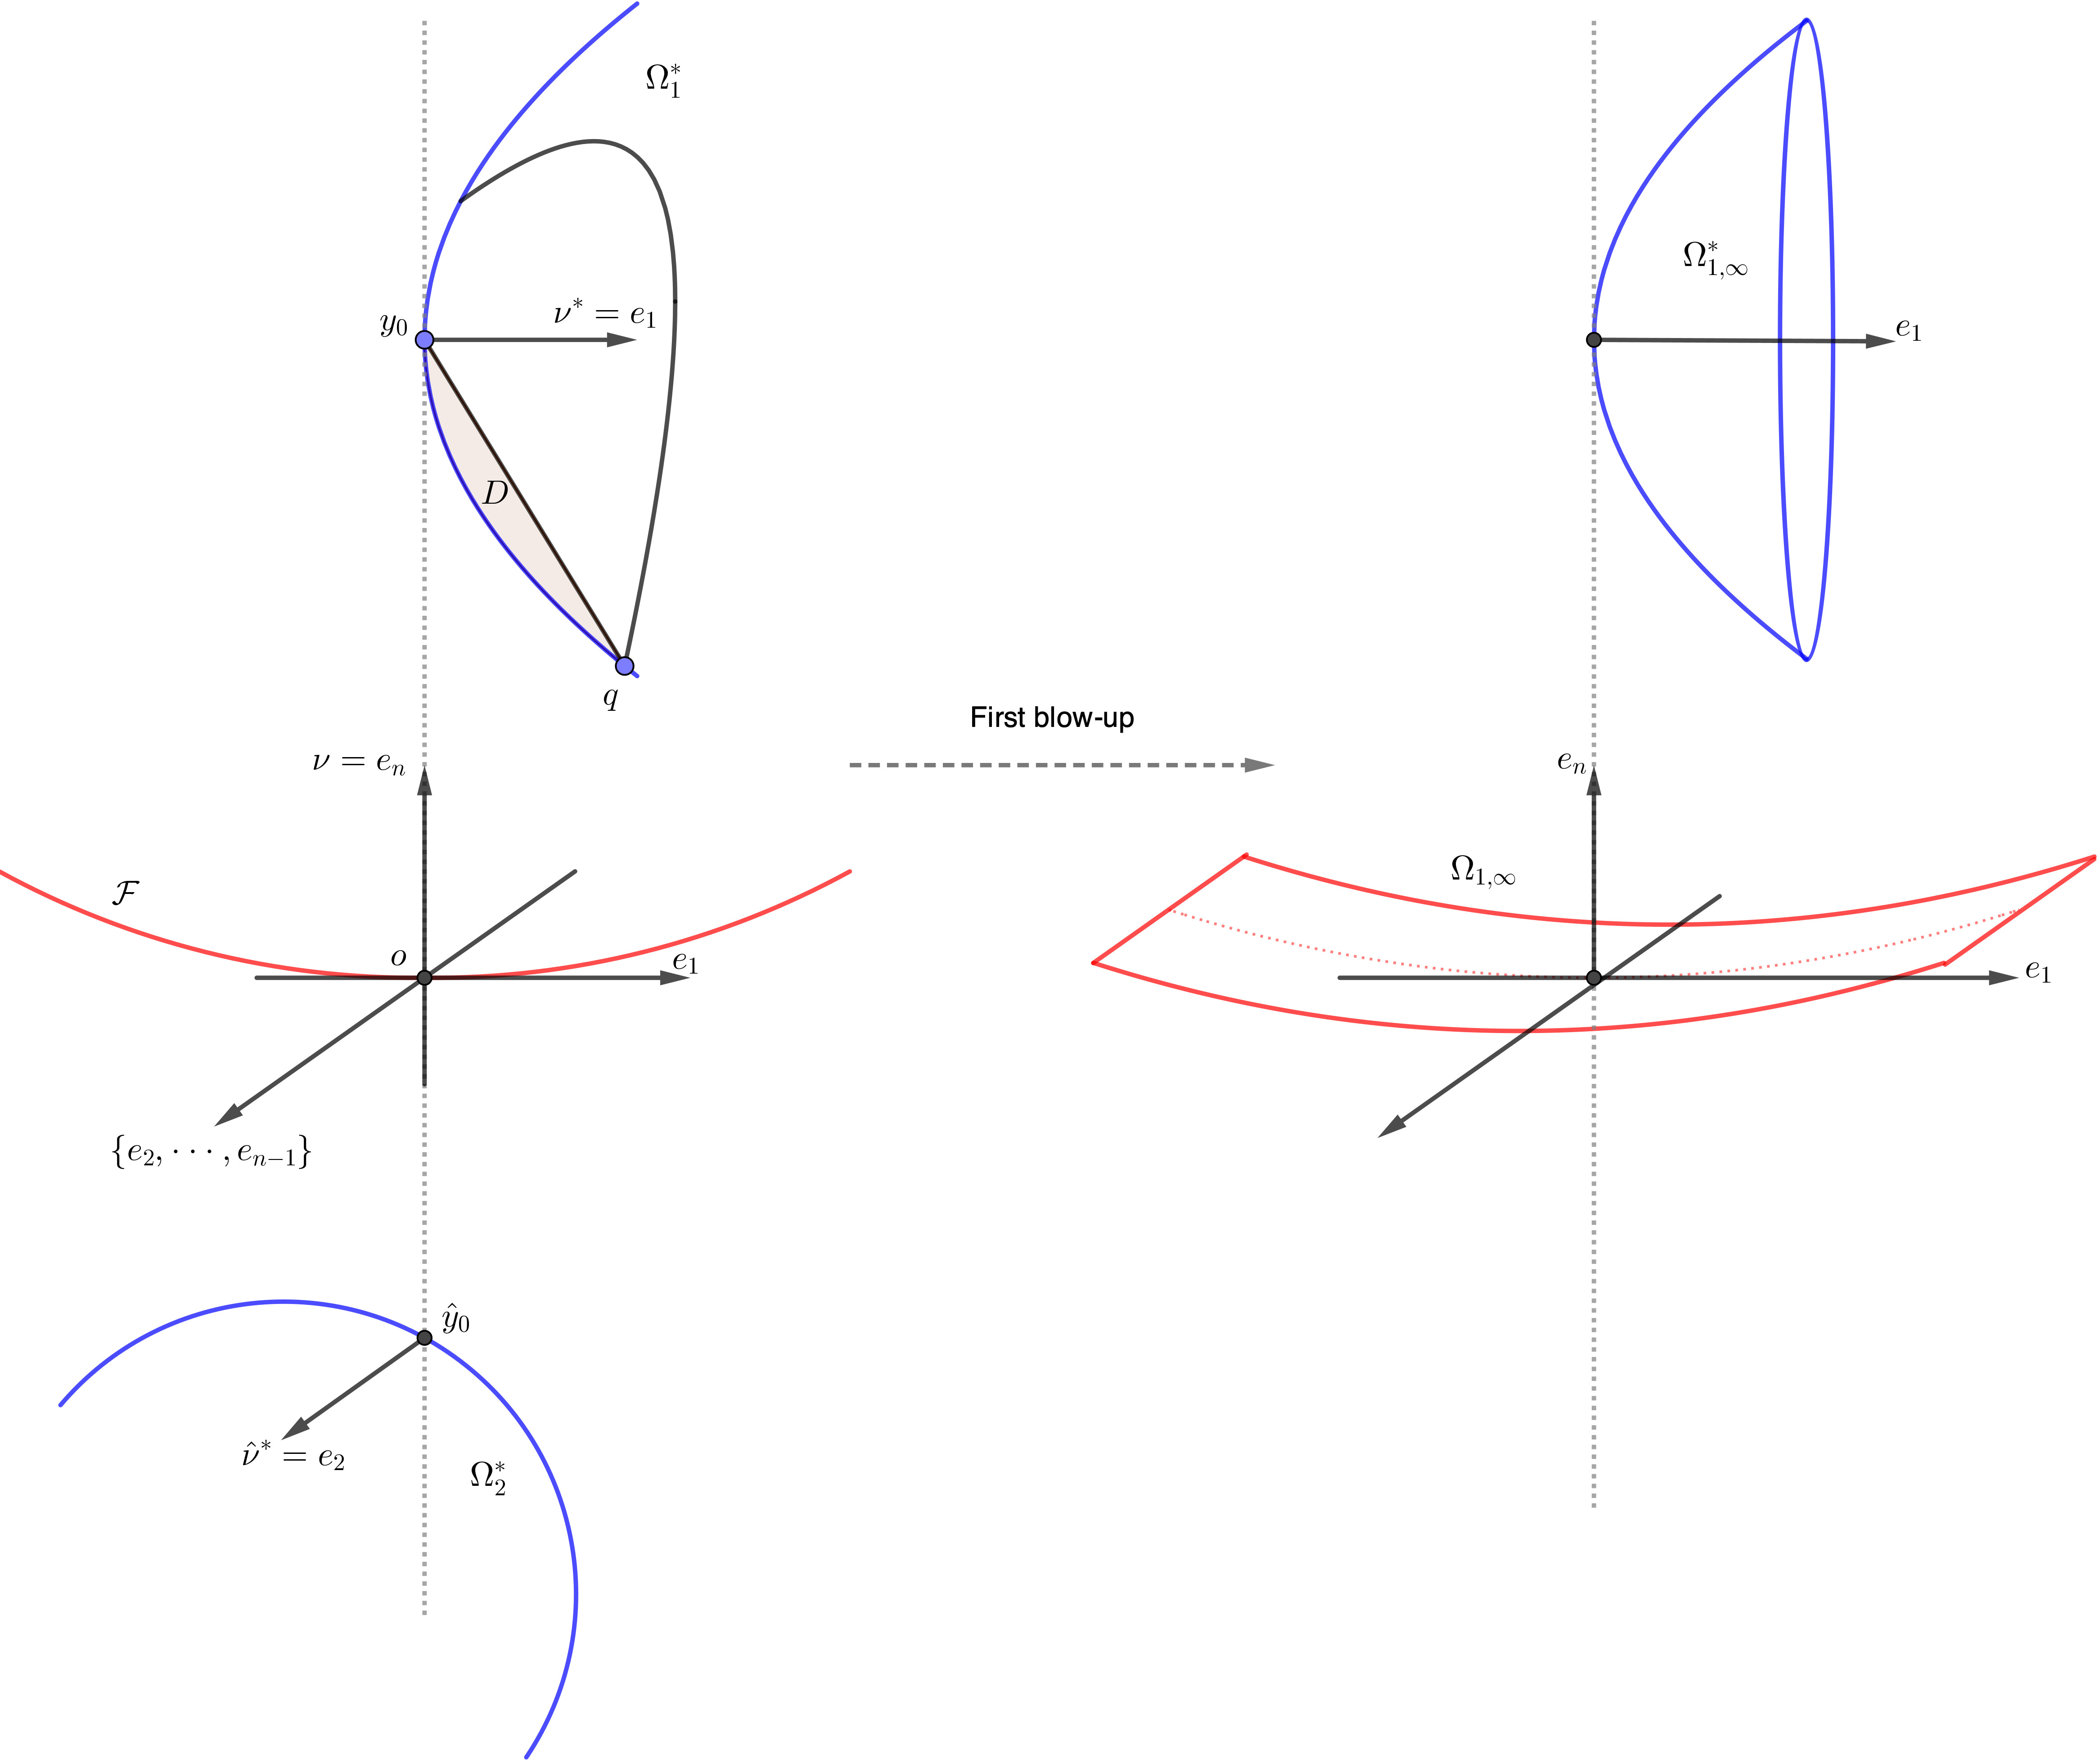
\includegraphics[scale=0.33]{3noncoplanar.png}
 \caption{The limit profile after the first blow-up. }
\end{figure}

\begin{thebibliography}{12}
 

\bibitem{Br1}
Y. Brenier, 
Polar factorization and monotone rearrangement of vector-valued functions. 
\emph{Comm. Pure Appl. Math.} 44 (1991), no. 4, 375--417.
 
\bibitem{C92}
 L. A. Caffarelli, 
 The regularity of mappings with a convex potential. 
 \emph{J. Amer. Math. Soc.} 5 (1992), 99--104.
 
\bibitem{C92b}
 L. A. Caffarelli, 
 Boundary regularity of maps with convex potentials. 
 \emph{Comm. Pure Appl. Math.} 45 (1992), 1141--1151.

\bibitem{C96}
L. A. Caffarelli, 
Boundary regularity of maps with convex potentials. II.
 \emph{Ann. of Math.} 144 (1996), 453--496.

 \bibitem{CM}  
 L. A. Caffarelli and R. J. McCann, 
 Free boundaries in optimal transport and Monge-Amp\`{e}re obstacle problems.
  \textit{Ann. of Math.} 171 (2010), 673--730.
  
\bibitem{CLL} 
S. Chen, Y. Li and J. Liu,
	Optimal (partial) transport between non-convex polygonal domains.
	Preprint, available at arXiv:2311.15655.

\bibitem{CL1}
S. Chen and J. Liu, 
Regularity of free boundaries in optimal transportation. 
Preprint, available at arXiv:1911.10790. 

\bibitem{CL2}
S. Chen and J. Liu, 
Global regularity in the Monge-Amp\`ere obstacle problem. 
Preprint, available arXiv:2307.00262.

\bibitem{CLW1} 
S. Chen, J. Liu and X.-J. Wang, 
Global regularity for the Monge-Amp\`ere equation with natural boundary condition.    
\textit{Ann. of Math.} (2) 194 (2021), no.3, 745--793.
 

\bibitem{CLW3}
S. Chen, J. Liu and X.-J. Wang,
$C^{2,\alpha}$ regularity of free boundaries in optimal transportation.  
\emph{Comm. Pure Appl. Math.} 77 (2024), 731--794. 

%\bibitem{DeFi}
%G. De Philippis and A. Figalli,
%The Monge-Amp\`ere equation and its link to optimal transportation.
%\emph{Bull. Amer. Math. Soc.} 51 (2014), 527--580.

\bibitem{D91} 
Ph. Delano\"e,
	    Classical solvability in dimension two of the second boundary value problem associated with the Monge-Amp\`ere operator.
	    \textit{Ann. Inst. Henri Poincar\'e, Analyse Non Lin\'eaire} 8 (1991), 443--457.

\bibitem{AF09} 
A. Figalli, 
A note on the regularity of the free boundaries in the optimal partial transport problem.
 \textit{Rend. Circ. Mat. Palermo} 58 (2009), no. 2, 283--286.
 	    
 \bibitem{AFi} 
 A. Figalli, 
 The optimal partial transport problem. 
  \textit{Arch. Ration. Mech. Anal.} 195 (2010), 533--560.
  
 \bibitem{FK1}  
 A. Figalli and Y.-H. Kim, 
 Partial regularity of Brenier solutions of the Monge–Amp\`ere equation. 
 \textit{Discrete Contin. Dyn. Syst.} 28 (2010), 559--565.

 \bibitem{GK}
 N. Guillen and J. Kitagawa,
 On the local geometry of maps with c-convex potentials.
 \textit{Calc. Var. Partial Differential Equations} 52 (2015), 345--387. 

 \bibitem{I} E. Indrei, Free boundary regularity in the optimal partial transport problem. 
 \textit{J. Funct. Anal.} 264 (2013), no. 11, 2497--2528.   
 

\bibitem{KM1} 
J. Kitagawa and R. McCann,
 Free discontinuities in optimal transport.
       \emph{Arch. Rational Mech. Anal.} 232 (2019), 1505--1541. 


\bibitem{SY}
   O. Savin and H. Yu,
    Regularity of optimal transport between planar convex domains. 
    \textit{Duke Math. J.} 169 (2020), 1305--1327.
   
   
\bibitem{U1} J. Urbas,
    On the second boundary value problem of Monge-Amp\`ere type.
      \textit{J. Reine Angew. Math.}  487 (1997), 115--124.


\bibitem{V1} C. Villani,
           \emph{Topics in optimal transportation}.  Grad. Stud. Math. 58,
          \textit{Amer. Math. Soc.}, 2003.

\bibitem{V2} C. Villani,
           \emph{Optimal transport, old and new}.  
           Springer, Berlin, 2006.

\end{thebibliography}
\end{document}
